\documentclass[tikz, border=5px]{standalone}
\usepackage{amsmath, amssymb, amsfonts, amscd}
\usepackage{amsthm, thmtools}
\usepackage{environ}
\usepackage{enumitem}
\usepackage{mathtools}
\usepackage{xcolor}
\newcommand{\vn}{\varnothing}
\DeclareMathOperator{\id}{id}
\usetikzlibrary{calc} % for coordinate calculations
\usetikzlibrary{automata,arrows} % for transition diagrams
\usetikzlibrary{decorations.pathreplacing}

% Colours
\definecolor{dBlue}{HTML}{4FB8DD}
\definecolor{dRed}{HTML}{FF2400}
\definecolor{dPurp}{HTML}{9932CC}
\definecolor{dPink}{HTML}{EE82EE}
\newcommand{\dRed}[1]{{\color{dRed}#1}}
\newcommand{\dBlue}[1]{{\color{dBlue}#1}}
\newcommand{\dPurp}[1]{{\color{dPurp}#1}}
\newcommand{\dPink}[1]{{\color{dPink}#1}}

\definecolor{grey}{HTML}{A9A9A9}


% To draw enddot in diagrams
% Params: Dot colour, scale
\tikzset{
    enddot/.style={
            circle,
            fill={#1},
            inner sep=0pt, % no inside-rectangle
            minimum size=5pt % min diameter 5pt
        },
    enddot/.default={black},
    enddot/scaled/.style 2 args={
            circle,
            fill={#1},
            inner sep=0pt, % no inside-rectangle
            minimum size=5/0.4*#2 pt % min diameter 5pt
        },
    enddot/scaled/.default={black}{0.4}
}

% To draw string in diagrams
% Params: Line colour, scale
\tikzset{
    string/.style={
            line width=1.2pt,
            {#1}
        },
    string/.default={black},
    string/scaled/.style 2 args={
            line width=1.2/0.4*#2 pt, % default very thick=1.2pt
            {#1}
        },
    string/scaled/.default={black}{0.4},
    round/.style={
            line cap=round
        },
}

% To draw box in diagrams (for nodes)
\tikzset{
    box/.style={
            draw,
            fill=white,
            rounded corners
        }
}

% Drawing braces
\tikzset{
    overbrace/.style={
            thick,
            decoration={
                    brace,
                    raise=1pt
                },
            decorate
        }
}
\tikzset{
    underbrace/.style={
            thick,
            decoration={
                    brace,
                    mirror,
                    raise=1pt
                },
            decorate
        }
}

\newcommand{\bigbox}[3]{%
    \draw[rounded corners, fill=white] ($ #2 $) rectangle node{#1} ($ #3 $);
}

% Centers inline tikz to the text
\tikzset{
    vcenter/.style={
            baseline={([yshift=-.5ex]current bounding box.center)}
        },
}

\newcommand{\squarecoord}{%
    \coordinate (top) at (2,4);
    \coordinate (topl) at (0,4);
    \coordinate (topr) at (4,4);
    %
    \coordinate (mid) at (2,2);
    %
    \coordinate (bot) at (2,0);
    \coordinate (botl) at (0,0);
    \coordinate (botr) at (4,0);
}

% Spawns two invisible points
\newcommand{\tikzfixsize}[2]{%
    \node at #1 {};
    \node at #2 {};
}

% Right wall
% Params: far right x-coordinate, height, width
\newcommand{\wallr}[3]{%
    % \draw[draw=none, fill=black!40, path fading = east]
    % (#1,#2) --
    % ++(-#3/2,0) --
    % ++(0,-#2) --
    % ++(#3/2,0) --
    % cycle;
    \shade [left color=transparent!50, right color=transparent!0, middle color=black!30] (#1,#2) rectangle (#1-#3,0);
}

% Left wall
% Params: far left x-coordinate, height, width
\newcommand{\walll}[3]{%
    % \draw[draw=none, fill=black!40]
    % (#1,#2) --
    % ++(#3,0) --
    % ++(0,-#2) --
    % ++(-#3,0) --
    % cycle;
    \shade [left color=transparent!50, right color=transparent!0, middle color=black!30] (#1,#2) rectangle (#1+#3,0);
}

% Draw a cap
\newcommand{\diagcap}[4][dRed]{%
    \draw[string=#1] (#2)
    to[out=90,in=180,looseness=1] (#3)
    to[out=0,in=90,looseness=1] (#4)
    ;
}

% Draw a cup
\newcommand{\diagcup}[4][dRed]{%
    \draw[string=#1] (#2)
    to[out=270,in=180,looseness=1] (#3)
    to[out=0,in=270,looseness=1] (#4)
    ;
}

% Draw a merge trivalent vertex
\newcommand{\diagmult}[5][dRed]{%
    \diagcap[#1]{#2}{#3}{#4};
    \path (#3) edge[string=#1] (#5);
}

% Draw a split trivalent vertex
\newcommand{\diagcomult}[5][dRed]{%
    \diagcup[#1]{#2}{#3}{#4};
    \path (#3) edge[string=#1] (#5);
}

\begin{document}

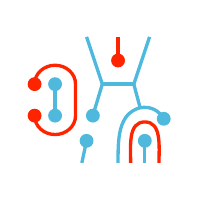
\begin{tikzpicture}[
        vcenter,
        scale=0.4,
    ]
    \squarecoord
    \tikzfixsize{(0,0)}{(4,4)}
    % \node (top) at ($(top)+(0,1)$) {};
    \node (mid) at ($(mid)+(0,.5)$) {};
    % centre blue
    \path[string=dBlue]
    ($(mid) + (-.5,0)$) edge ($(mid) + (.5,0)$)
    ($(mid) + (-.5,0)$) edge ($(top) + (-1,0)$)
    ($(mid) + (.5,0)$) edge ($(top) + (1,0)$)
    ($(mid) + (-.5,0)$) edge ($(mid) + (-.8,-1)$)
    ($(mid) + (.5,0)$) edge ($(mid) + (.7,-.75)$);
    \draw[string=dBlue] (bot)
    to[out=90,in=195] ($(mid) + (.7,-.75)$)
    to[out=10,in=120] ($(mid) + (.7,-.75) + (.75,-.35)$);
    \node[enddot=dBlue] at ($(mid) + (-.8,-1)$) {};
    \node[enddot=dBlue] at ($(mid) + (.7,-.75) + (.75,-.35)$) {};
    % red cap
    \draw[string=dRed] ($(bot) + (.4,0)$)
    to[out=90,in=180] ($(bot) + (.85,1.3)$)
    to[out=0,in=90] ($(bot) + (1.3,0)$);
    % stalactite and stalagmite
    \path
    ($(bot) + (-1.15,0)$) edge[string=dBlue] ($(bot) + (-1,.7)$)
    (top) edge[string=dRed] ($(top) + (0,-.75)$)
    ($(bot) + (.85,0)$) edge[string=dBlue] ($(bot) + (.85,.7)$);
    \node[enddot=dBlue] at ($(bot) + (-1,.7)$) {};
    \node[enddot=dRed] at ($(top) + (0,-.75)$) {};
    \node[enddot=dBlue] at ($(bot) + (.85,.7)$) {};
    % left barbells
    \path[string=dBlue] (0,1.5) edge (0,2.5);
    \draw[string=dRed] (-.65,1.5)
    to[out=270,in=180] (0,.9)
    to[out=0,in=270] (.65,1.5)
    to (.65,2.5)
    to[out=90,in=0] (0,3.1)
    to[out=180,in=90] (-.65,2.5);
    \node[enddot=dBlue] at (0,1.5) {};
    \node[enddot=dBlue] at (0,2.5) {};
    \node[enddot=dRed] at (-.65,1.5) {};
    \node[enddot=dRed] at (-.65,2.5) {};
\end{tikzpicture}

\end{document}
